%!TEX encoding = UTF-8 Unicode
\documentclass{beamer}
\usepackage{amsmath,amsthm,amssymb}
\usepackage{CJKutf8}
\usepackage{graphicx}
\usepackage{hyperref}
\usepackage{pstricks-add}
\useoutertheme{sidebar}

\begin{document}
\begin{CJK}{UTF8}{bsmi}
\title{期中小考詳解}
\author[何震邦]{何震邦 \href{mailto:jdh8@ms63.hinet.net}{\textless jdh8@ms63.hinet.net\textgreater}\\
    \href{http://creativecommons.org/licenses/by-sa/3.0/tw/deed.zh\textunderscore TW}{\includegraphics{by-sa.eps}}}
\date{2012 年 10 月 31 日}
\maketitle

\section{第 1 題}
\begin{frame}{第 1 題}
  In a study of five industrial areas, a researcher obtained these data relating the average number of units of a certain
  pollutant in the air and the number of incidences (per 100\,000 people) of a certain disease:
  \begin{center}
    \begin{tabular}{c|ccccc}
      Units of pollutant       & 3.4& 4.6& 5.2& 8.0& 10.7\\
      \hline
      Incidences of the disease& 48 & 52 & 58 & 70 & 96
    \end{tabular}
  \end{center}
  Find the equation of the least-square line $y = Ax + B$ (to two decimal places.)
  \centerline{Given that $A = \dfrac{n \sum xy - \sum x \sum y}{n \sum x^2 - (\sum x)^2}$ and $B
      = \dfrac{\sum y - A \sum x}{n}.$}
\end{frame}

\begin{frame}{第 1 題詳解}
  \begin{solution}
    \begin{center}
      \begin{tabular}{crrrr}
	      &\multicolumn1c{$x$}& \multicolumn1c{$y$}& \multicolumn1c{$x^2$}& \multicolumn1c{$xy$}\\
	\hline
	      & 3.4&  48& 11.56& 163.2\\
	      & 4.6&  52& 21.16& 239.2\\
	      & 5.2&  58& 27.04& 301.6\\
	      & 8.0&  70& 64.00& 560.0\\
	      &10.7&  96&114.49&1027.2\\
	\hline
	$\sum$&31.9& 324&238.25&2291.2
      \end{tabular}
    \end{center}
    \[A = \frac{n \sum xy - \sum x \sum y}{n \sum x^2 - (\sum x)^2},\quad B = \frac{\sum y - A \sum x}{n}\]
    \[A = \frac{1120.4}{173.64},\quad B = 0.2 \left( 324 - 31.9 \left( \frac{1120.4}{173.64} \right) \right)\]
    \[y = 6.45 x + 23.63\]
  \end{solution}
\end{frame}

\section{第 2 題}
\begin{frame}{第 2 題}
  Given $f(x) = x^3 - 3x^2 + 3$, use definition $\displaystyle f'(x) = \lim_{h\to0} \frac{f(x+h) - f(x)}{h}$ to find $f'(x)$.
  \begin{solution}
    \begin{align*}
      f'(x) &= \lim_{h\to0} \frac{(x+h)^3 - 3 \left(x+h \right)^2 + 3 - \left( x^3 - 3x^2 + 3 \right)}{h}\\
	&= \lim_{h\to0} \frac{3x^2 h + 3xh^2 + h^3 - 3 \left( 2xh + h^2 \right)}{h}\\
	&= \lim_{h\to0} \left( 3x^2 + 3xh + h^2 - 3 \left( 2x + h \right) \right)\\
	&= 3x^2 - 6x
    \end{align*}
  \end{solution}
\end{frame}

\section{第 3 題}
\begin{frame}{第 3 題}
  Find the equation of the tangent of the curve $\left( x^2 + 3 \right) (x - 3)^{\frac12}$ at $x = 4$.
  \begin{solution}
    設 $f(x) := \left( x^2 + 3 \right) \sqrt{x - 3}$
    \begin{align*}
      f'(x) &= 2x \sqrt{x-3} + \frac{x^2 + 3}{2 \sqrt{x-3}}\\
      f(4) &= 19\\
      f'(4) &= 8 + \frac{19}{2} = \frac{35}{2}
    \end{align*}
    所以切線方程式為
    \[y - 19 = \frac{35 \left( x-4 \right)}{2}\]
  \end{solution}
\end{frame}

\section{第 4 題}
\begin{frame}{第 4 題}
  Consider a curve $f(x) = \dfrac{(x+2)}{(x-3)^{0.5}}$. Find $f'(1)$ and $f''(1)$.
  \begin{solution}
    \begin{align*}
      f'(x) &= \frac{1}{\sqrt{x-3}} - \frac{x+2}{2 \left( x-3 \right)^{\frac32}}\\
      f''(x) &= \frac{3 \left( x+2 \right)}{4 \left( x-3 \right)^{\frac52}} - \frac{1}{(x-3)^{\frac32}} \\
      f'(1) &= -\frac{\textup i}{\sqrt2} - \frac{3\,\textup i}{2^{\frac52}} = -\frac{7\,\textup i}{2^{\frac52}}\\
      f''(1) &= -\frac{\textup i}{2^{\frac32}} - \frac{9\,\textup i}{2^{\frac92}} = -\frac{17\,\textup i}{2^{\frac92}}
    \end{align*}
  \end{solution}
\end{frame}

\section{第 5 題}
\begin{frame}{第 5 題}
  Sketch the graph of $\dfrac{3x^5 - 20x^3}{32}$ and also find the relative extreme points and inflection points at the
  interval of $[-1, 1]$.
  \begin{solution}
    注意本題是奇函數
    \begin{align*}
      f(x) &= \frac{3x^5 - 20x^3}{32}\\
      f'(x) &= \frac{15x^4 - 60x^2}{32}\\
      f''(x) &= \frac{15x^4 - 30x^2}{8}
    \end{align*}
  \end{solution}
\end{frame}

\begin{frame}{第 5 題詳解}
  \begin{enumerate}
    \item 解導函數的零點,找到臨界點為 $(0,0)$
    \item 解二階導函數的零點,找到可能的反曲點為 $(0,0)$
  \end{enumerate}
  \begin{center}
    \psset{unit=2}
    \begin{pspicture}(-1,-1)(1,1)
      \psaxes(0,0)(-1,-1)(1,1)
      \psplot[plotstyle=curve]{-1}{1}{x x mul dup x mul exch 3 mul 20 sub mul 32 div}
      \psdot(0,0)
      \uput[45](0,0){反曲點 $(0,0)$}
      \uput[0](1,-0.53125){$\left( 1, -\dfrac{17}{32} \right)$}
      \uput[180](-1,0.53125){$\left( -1, \dfrac{17}{32} \right)$}
    \end{pspicture}
  \end{center}
\end{frame}

\section{第 6 題}
\begin{frame}{第 6 題}
  Given $f(x) = 2^{x^2 + 1}$, find $\dfrac{df(x)}{dx}$.
  \begin{solution}
    \begin{align*}
      \ln |f(x)| &= (\ln 2) \left( x^2 + 1 \right)\\
      \frac{f'(x)}{f(x)} &= \left( 2 \ln 2 \right) x\\
      f'(x) &=  \left( \ln 2 \right) x\,2^{x^2 + 2}
    \end{align*}
  \end{solution}
\end{frame}

\section{第 7 題}
\begin{frame}{第 7 題}
  Find the equation of the tangent line to the curve $x^2 + 2xy + y^2 = 16$ at $(1,3)$.
  \begin{solution}
    \[2x + 2 \left( y + xy' \right) + 2yy' = 0\]
    \[\left( x+y \right) y' = -x - y\]
    \[y' = -1\]
    故切線方程式為
    \[y - 3= -(x - 1)\]
  \end{solution}
\end{frame}

\begin{frame}{第 7 題另解}
  \begin{solution}
    \[(x+y)^2 = 16\]
    \[(x+y+4) \left( x+y-4 \right) = 0\]
    圖形為兩平行直線。因點 $(1,3)$ 在直線 $x+y-4=0$ 上,故切線方程式為
    \[x+y-4 = 0\]
  \end{solution}
\end{frame}

\section{第 8 題}
\begin{frame}{第 8 題}
  Use the differentials to approximate the quantity $\sqrt{5.6}$ to four decimal places.
  \begin{solution}
    \begin{align*}
      f(x) &\approx f(c) + f'(c) \left( x-c \right)\\
      \sqrt x &\approx \sqrt c + \frac{x-c}{2 \sqrt c}
    \end{align*}
    \begin{align*}
      \sqrt{5.6} &\approx 2 + \frac{5.6 - 4}{4} = 2.4\\
      \sqrt{5.6} &\approx 2.4 + \frac{5.6 - 5.76}{4.8} = \frac{71}{30} \approx 2.36667\\
      \sqrt{5.6} &\approx \frac{71}{30} + \frac{5.6 - \frac{5041}{900}}{71/15} = \frac{71}{30} - \frac{1}{4260} \approx 2.3664
    \end{align*}
  \end{solution}
\end{frame}

\begin{frame}{第 8 題另解}
  \begin{solution}
    \begin{columns}
      \begin{column}{0.5\textwidth}
	\begin{center}
	  \begin{tabular}{@{}c@{}c@{}c@{}c@{}c@{} r@{}r@{}c@{}r@{}r@{} r@{}r@{}r@{}}
	   & & & & &       &2&.& &3& 6& 6& 4\\
		     \cline{7-13}
	  2& & & & &$\surd$&5&.&6& \\
	  2& & & & &       &4& & & \\
	  \cline{1-2}\cline{7-13}
	  4&3& & & &       &1& &6&0\\
	   &3& & & &       &1& &2&9\\
	  \cline{1-3}\cline{7-13}
	  4&6&6& & &       & & &3&1&00\\
	   & &6& & &       & & &2&7&96\\
	  \cline{1-4}\cline{9-13}
	  4&7&2&6& &       & & & &3&04&00\\
	   & & &6& &       & & & &2&83&56\\
	  \cline{1-5}\cline{10-13}
	  4&7&3&2&4&       & & & & &20&44&00\\
	   & & & & &       & & & & &18&92&96\\
		     \cline{11-13}
	   & & & & &       & & & & & 1&51&04
	  \end{tabular}
	\end{center}
      \end{column}
      \begin{column}{0.5\textwidth}
	\begin{align*}
	  f(x) &\approx f(c) + f'(c) \left( x-c \right)\\
	  \sqrt x &\approx \sqrt c + \frac{x-c}{2 \sqrt c}\\
	  \sqrt{5.6} &\approx 2.3664 + \frac{5.6 - (2.3664)^2}{2 \left( 2.3664 \right)}\\
	    &\approx 2.3664
	\end{align*}
      \end{column}
    \end{columns}
  \end{solution}
\end{frame}

\section{第 9 題}
\begin{frame}{第 9 題}
  When a person coughs, the trachea (windpipe) contracts, allowing the air to be expelled at a maximum velocity. It can be
  shown that during a cough, the velocity $v$ of airflow is given by the function $v = f(r) = kr^2 \left( R-r \right)$, where
  $r$ is the radius of the trachea (in centimeters) during a cough, $R$ is the normal radius of the trachea (in centimeters),
  and $k$ is a positive constant that depends on the length of the trachea. Find the radius $r$ for which the velocity of
  airflow is greatest.
\end{frame}

\begin{frame}{第 9 題詳解}
  \begin{solution}
    \begin{align*}
      f(r) &= k \left( Rr^2 - r^3 \right)\\
      f'(r) &= k \left( 2Rr - 3r^2 \right)\\
      f''(r) &= k \left( 2R - 6r \right)
    \end{align*}
    \[f'(r) = 0 \;\Leftrightarrow\; r = 0\textup{(不合)} \vee r = \frac{2R}{3}\]
    \[f'' \left( \frac{2R}{3} \right) = -2kR < 0 \;\Rightarrow\; r = \frac{2R}{3}\]
  \end{solution}
\end{frame}

\section{第 10 題}
\begin{frame}{第 10 題}
  \small
  Several mathematical stories originated with the second wedding of the mathematician and astronomer Johannes Kepler. Here
  is one: While shopping for wine for his wedding, Kepler noticed that the price of a barrel of wine (here assumed to be a
  cylinder) was determined solely by the length $d$ of a dipstick that was inserted diagonally through a hole in the top of
  the barrel to the edge of the base of the barrel (see figure). Kepler realized that this measurement does not determine the
  volume of the barrel and that for a fixed value of $d$. The volume varies with the radius $r$ and height $h$ of the barrel.
  For a fixed value of $d$, what is the ratio $r/h$ that maximizes the volume of the barrel?
  \begin{center}
    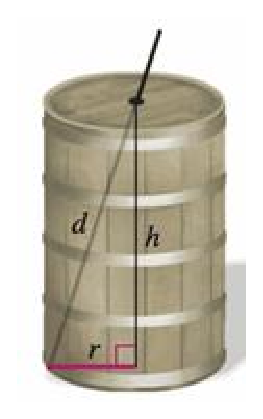
\includegraphics[height=0.3\textheight]{barrel.eps}
  \end{center}
\end{frame}

\begin{frame}{第 10 題詳解}
  \begin{solution}
    設體積為 $V$,則
    \[V = \pi r^2 h = \pi h \left( d^2 - h^2 \right) = \pi \left( d^2 h - h^3 \right)\]
    \begin{align*}
      \frac{dV}{dh} &= \pi \left( d^2 - 3h^2 \right)\\
      \frac{d^2V}{dh^2} &= -6\pi h < 0
    \end{align*}
    \[\frac{dV}{dh} = 0 \;\Leftrightarrow\; h = \pm\frac{d}{\sqrt3}\textup{(負不合)}\]
    \[r = \sqrt{\frac23}d,\quad \frac rh = \sqrt2\]
  \end{solution}
\end{frame}

\begin{frame}
  \begin{center}
    \huge Thanks for your attention!
  \end{center}
\end{frame}

\end{CJK}
\end{document}
